
In the analysis, the $\Pqt \Paqt$ background is estimated from data. Additional
plots supporting the robustness of the procedure are presented below.
The comparison of $\EM$ and $(\EE+\MM)$ distributions using Powheg + Pythia top MC shows
an excellent agreement, as depicted in Figure~\ref{figap:emumc1}
for several variables after different steps of the selection. A similar agreement
is observed in Figure~\ref{figap:emudata1}, which compares the 2012 $\EM$ data to Powheg + Pythia top MC.
Figure~\ref{figap:emu_ll_comp_met} displays the MET significance distribution
for dilepton data compared to the sum of Drell-Yan Monte Carlo
plus $\EM$ data for events with two b-tags (1 JPM + 1 JPL), and the dijet
invariant mass (right) for $\EE + \MM$ and $\EM$ data for events outside the leptonic $Z$ mass window,
show again very good agreement.

\begin{figure}[!htb]
  \centerline{
    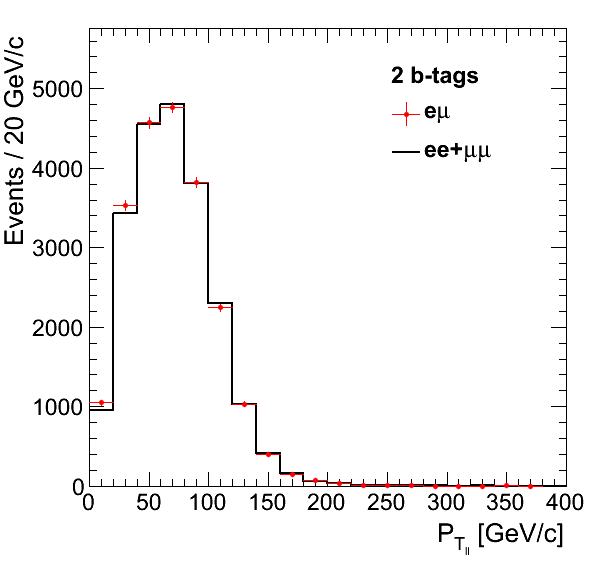
\includegraphics[width=0.43\textwidth]{plots/emu_mc_ZllPt_5}
    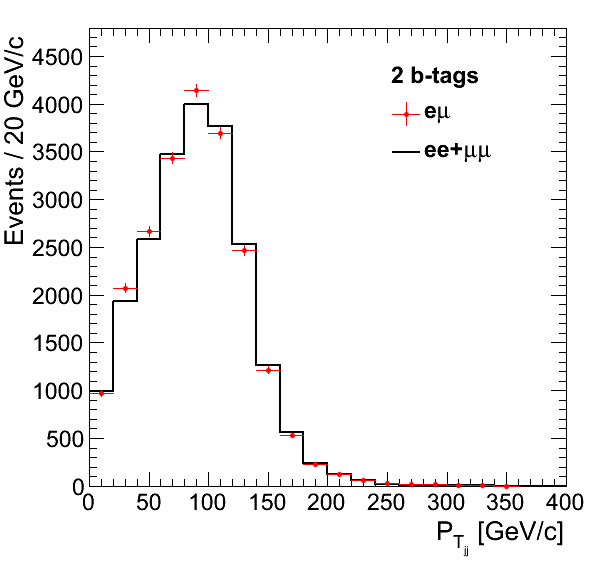
\includegraphics[width=0.43\textwidth]{plots/emu_mc_ZjjPt_5}
  }
  \centerline{
    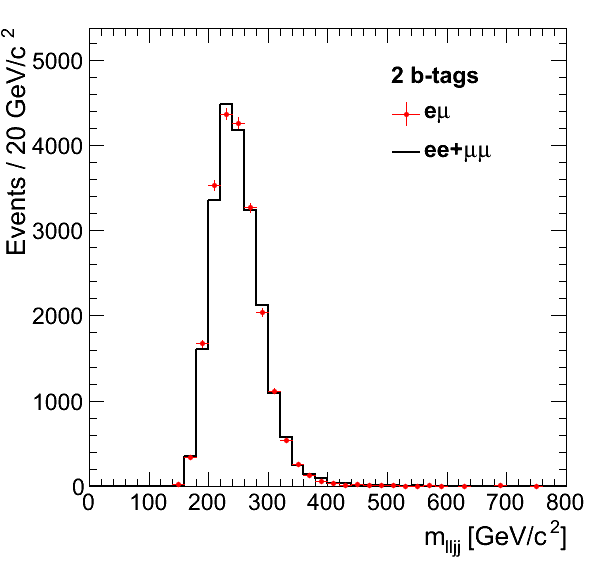
\includegraphics[width=0.43\textwidth]{plots/emu_mc_HiggsMass_5}
    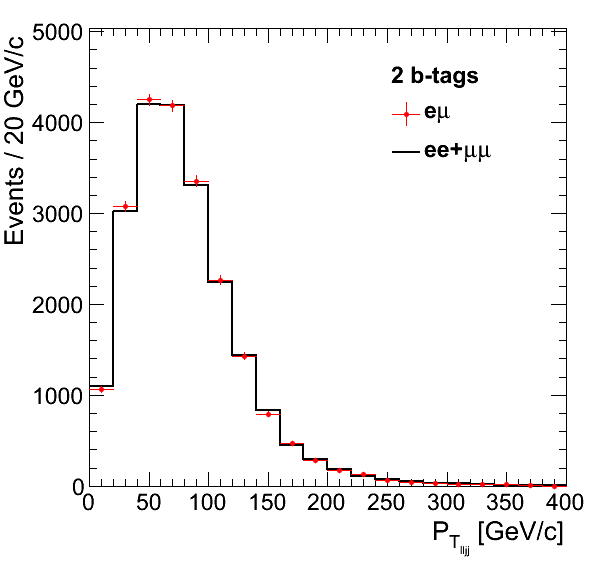
\includegraphics[width=0.43\textwidth]{plots/emu_mc_HiggsPt_5}
  }
  \caption{\label{figap:emumc1} Powheg + Pythia top MC $\EM$ to
    $(\EE+\MM)$ comparison for several variables after different
    steps of the selection, as specified in the legends. Top:
    dilepton (left) and dijet transverse momentum (right). Bottom:
    dilepton + dijet ``Higgs'' invariant mass (left) and transverse
    momentum (right).}
\end{figure} 

\begin{figure}[!htb]
  \centerline{
    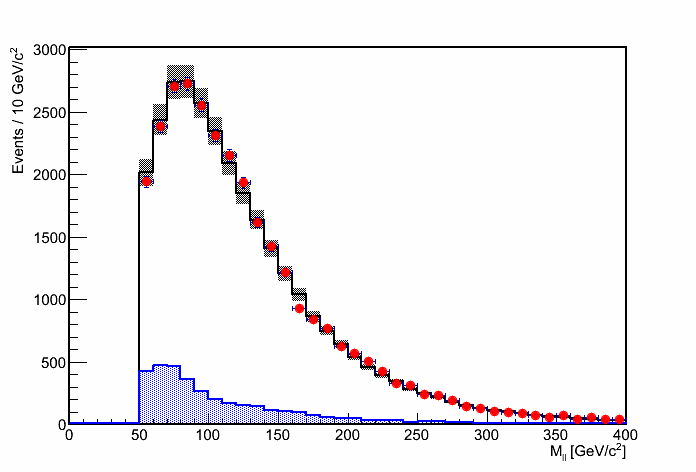
\includegraphics[width=0.49\textwidth]{plots/emu_zllm1_0}
    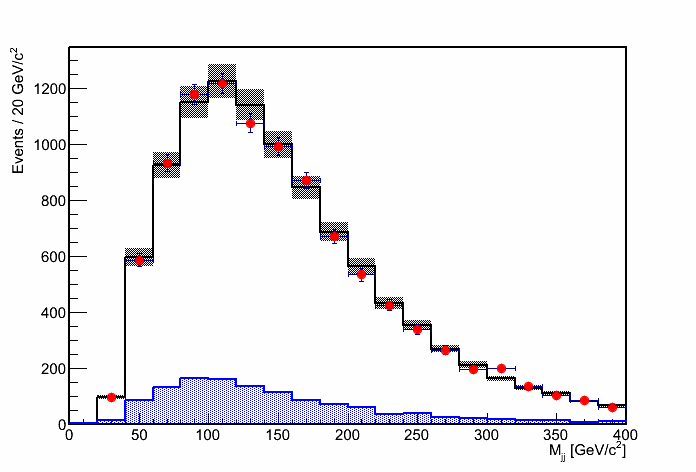
\includegraphics[width=0.49\textwidth]{plots/emu_zjjm2_0}
  }
  \centerline{
    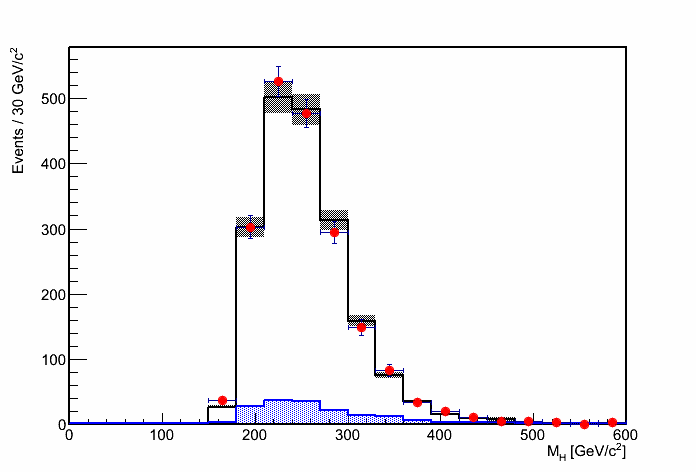
\includegraphics[width=0.49\textwidth]{plots/emu_hm3_1}
    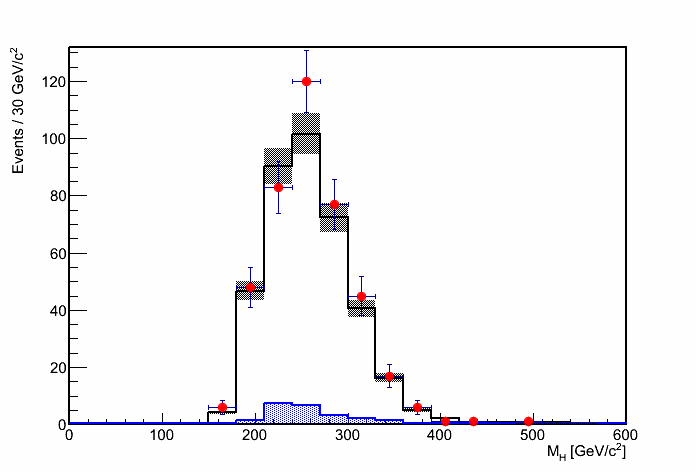
\includegraphics[width=0.49\textwidth]{plots/emu_hm3_3}
  }
  \caption{\label{figap:emudata1}Comparison of 2012 $\EM$ data to
    Powheg + Pythia top MC, corresponding to an integrated luminosity
    of 19.6 fb$^{-1}$. Red dots are $\EM$ data; white histogram top
    Monte Carlo; blue histogram other small backgrounds.  Top:
    dilepton invariant mass (left) and dijet invariant mass
    (right). Bottom: ``Higgs'' invariant mass for events with 1
    JPL b-tag (left), and two (1 JPM + 1 JPL) b-tags and MET
    significance $< 10$ (right).}
\end{figure}

Next, the data-driven evaluation of the $\Pqt \Paqt$ background is compared to an alternative
method based on top simulation only. 
Figure~\ref{figap:emudata2} compares the previous $\EM$ data distributions to the prediction of
Powheg + Pythia top MC normalized to the NLO $\Pqt \Paqt$ cross-section.
The gray area represents the systematic error (including luminosity, lepton trigger and ID efficiencies,
b-tagging efficiency, mistag efficiency, and pile-up uncertainties; no contribution from normalization) of the MC
prediction. With the 19.6~\fbinv{}, the statistical errors of the $\EM$ data points compare well
to the size of the gray boxes. In addition, the $\Pqt \Paqt$ MC underestimates the normalization of the
$\EM$ data by $20\%$ before b-tagging ($12\%$ for events with  2 b-tagged jets). Based on this comparison,
we chose to use the data-driven estimation.

\begin{figure}[!htb]
  \centerline{
    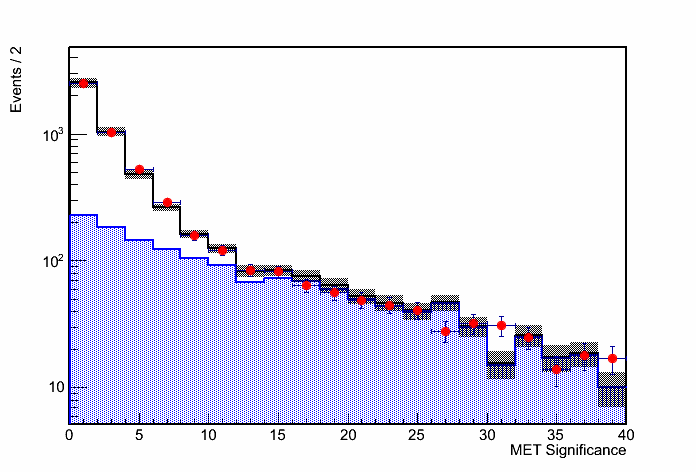
\includegraphics[width=0.55\textwidth]{plots/emu_mets1l_2dy}
    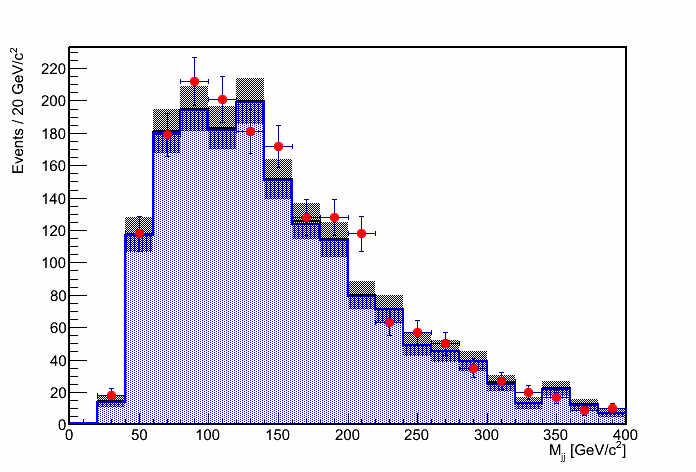
\includegraphics[width=0.55\textwidth]{plots/emu_zjjm2_2dy_side}
  }
  \caption{ \label{figap:emu_ll_comp_met} MET significance distribution
    for dilepton data compared to the sum of Drell-Yan Monte Carlo
    plus $\EM$ data for events with two btags (left).
    Dijet invariant mass (right) for $\EE + \MM$ and $\EM$
    data for events outside the leptonic $Z$ mass window, with two
    b-tags, and MET significance $>$ 8. Other cuts are
    detailed in the text.
    Red dots are $\EE+\MM$ data; white
    histogram Drell Yan Monte Carlo; blue histogram $\EM$ data (plus
    other small backgrounds).}

\end{figure}

\begin{figure}[!htb]
  \centerline{
    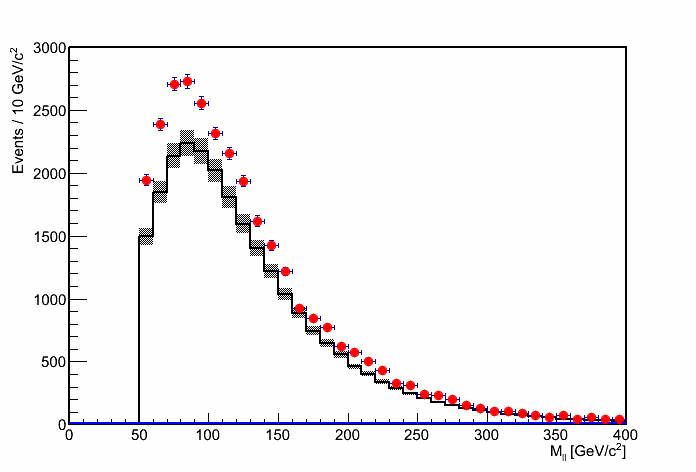
\includegraphics[width=0.49\textwidth]{plots/emu_zllm1_4}
    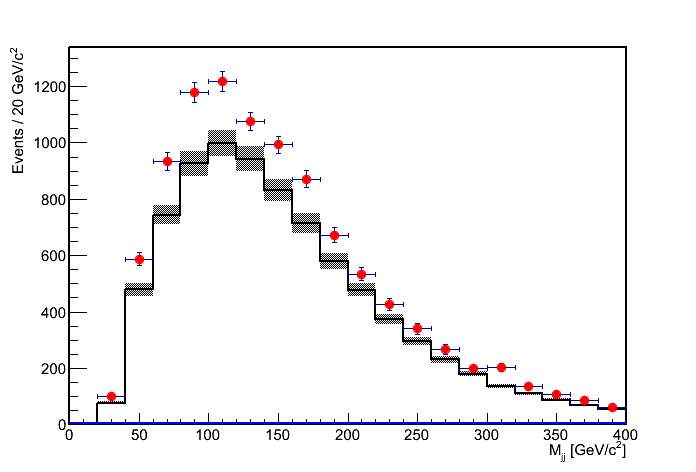
\includegraphics[width=0.49\textwidth]{plots/emu_zjjm2_4}
  }
  \centerline{
    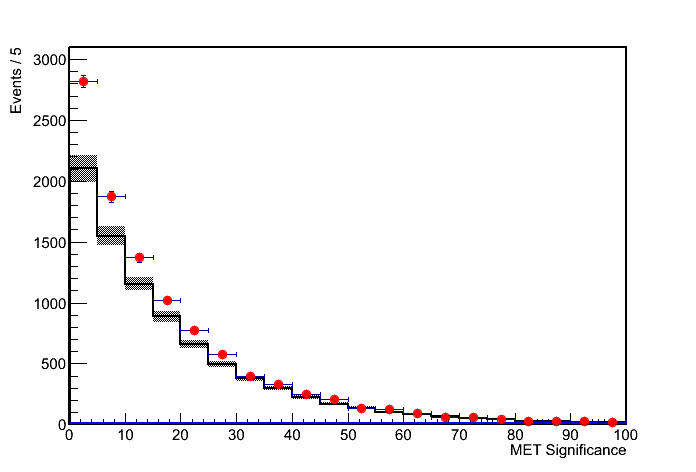
\includegraphics[width=0.49\textwidth]{plots/emu_mets2_4}
    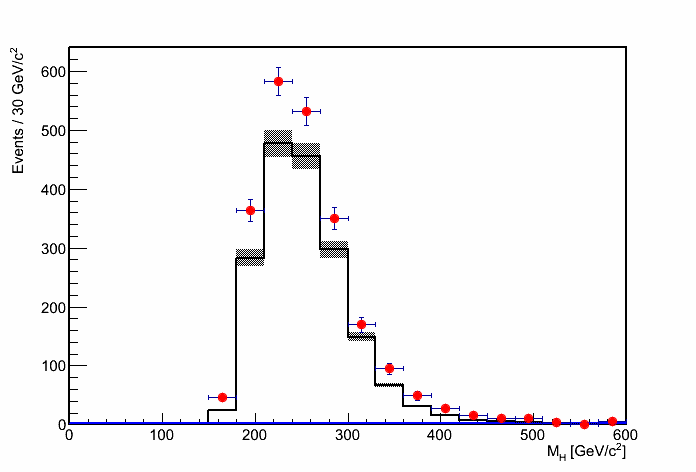
\includegraphics[width=0.49\textwidth]{plots/emu_hm3_4}
  }
  \caption{\label{figap:emudata2}Comparison of 2012 $\EM$ data to
    Powheg + Pythia top MC normalized to the $\Pqt \Paqt$ NLO cross-section.
    Red dots are $\EM$ data; white histogram top Monte Carlo. Top:
    dilepton invariant mass (left) and dijet invariant mass
    (right). Bottom: MET significance (left), and ``Higgs'' invariant
   mass  (right).}
\end{figure}

